\begin{frame}{Training und Ressourcen}
\scriptsize
\resizebox{\textwidth}{!}{%
\begin{tabular}{l l r r r l}
\toprule
Lauf & Modelle & Bilder & Epochen & Batch & GPU \\
\midrule
Red20-Smoke & YOLOv8m, Faster R-CNN, RetinaNet, FCOS & ca. 644 & 1 & 2 & AMD Radeon PRO W7800 48GB \\
Red6-Finallauf & YOLOv8m, FCOS, Faster R-CNN & 2.147 & 10 & 2 & AMD Radeon PRO W7800 48GB \\
\bottomrule
\end{tabular}}
\vspace{0.5em}
\begin{tabularx}{\textwidth}{>{\raggedright\arraybackslash}p{0.28\textwidth} r r X}
\toprule
Modell & Trainingszeit & Größe & Trainingshinweis \\
\midrule
YOLOv8m red6 ep10 & 16,1 min & 50 MB & Precision 0,839; Recall 0,579; mAP50 0,660 im YOLO-Run \\
FCOS red6 ep10 & ca. 58 min & 123 MB & Mean Loss 1,243 $\rightarrow$ 0,735 \\
Faster R-CNN red6 ep10 & läuft & -- & gleicher Datensatz; Werte werden nach Training/Evaluation ergänzt \\
\bottomrule
\end{tabularx}
\vspace{0.15em}
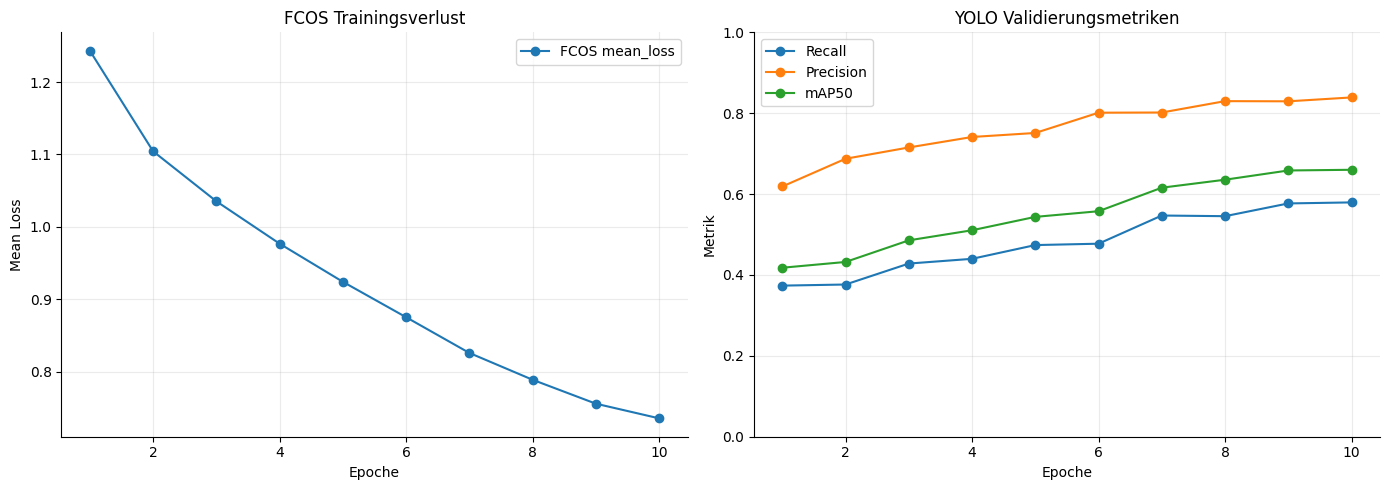
\includegraphics[width=\textwidth,height=0.24\textheight,keepaspectratio]{imglib/face_model_lab/lernkurven_loss_accuracy.png}
\vspace{0.05em}
\tiny Rohdaten: Trainingshistorien und YOLO-Results aus `model_results/` und `trained_models/yolo_runs/`.
\end{frame}
